\documentclass[aspectratio=169,10pt]{beamer}
\usetheme{default}
\setbeamertemplate{navigation symbols}{}
\setbeamertemplate{footline}{\hspace{3mm}\textcolor{gray}{\tiny Smart HVAC Temperature Control and Fault Detection}\hfill\textcolor{gray}{\tiny\insertframenumber\,/\,\inserttotalframenumber}\hspace{3mm}\vspace{2mm}}
\definecolor{accent}{HTML}{1F4E9C}
\setbeamercolor{frametitle}{fg=accent}
\setbeamercolor{title}{fg=accent}
\setbeamercolor{structure}{fg=accent}
\setbeamerfont{frametitle}{series=\bfseries}
\usepackage[utf8]{inputenc}
\usepackage{booktabs}
\usepackage{siunitx}
\usepackage{tikz}
\usetikzlibrary{arrows.meta,positioning,calc,fit}
\graphicspath{{../figures/}}

\title{Smart HVAC Temperature Control and Fault Detection}
\subtitle{MATLAB/Simulink modelling and laboratory-scale hardware}
\author{Somanshu Juneja (B24354) \and Ridhi Garg (B24348) \and Pramukto Mandal (B24347)}
\institute{EE302 Control Systems Laboratory \,\textbullet\, Group 2 \,\textbullet\, Problem Statement 4\\ IIT Mandi}
\date{November 2026}

\tikzset{
  blk/.style={draw, rounded corners=1pt, minimum height=6mm, minimum width=10mm, align=center, fill=accent!5},
  sum/.style={draw, circle, inner sep=1.2pt},
  box/.style={draw, rounded corners=1pt, align=center, minimum height=7mm, inner sep=2pt, fill=accent!5},
  lab/.style={font=\tiny, inner sep=1pt}}

\begin{document}

\begin{frame}
\titlepage
\end{frame}

% ---------------------------------------------------------------
\begin{frame}{Objectives}
\begin{columns}[T]
\column{0.56\textwidth}
\begin{enumerate}
\item \textbf{Thermal model} of the chamber, implemented in Simulink
\item \textbf{Controller comparison}: ON-OFF vs.\ PI\\ rise time, settling time, overshoot, steady-state error
\item \textbf{Real-time hardware} control with logged reference, temperature and command
\item \textbf{Disturbance response}: change the ventilation path, compare with simulation
\item \textbf{Fault detection}: restricted airflow, fan failure, sensor bias; normal vs.\ faulted energy and duty
\end{enumerate}
\column{0.40\textwidth}
\small
\textbf{Approach}\\
Identify a model from a step test \(\to\) tune PI \(\to\) run the same experiments in Simulink and on hardware \(\to\) detect faults from the gap between measured and predicted temperature.
\end{columns}
\end{frame}

% ---------------------------------------------------------------
\begin{frame}{System design: hardware}
\begin{columns}[c]
\column{0.55\textwidth}
\centering
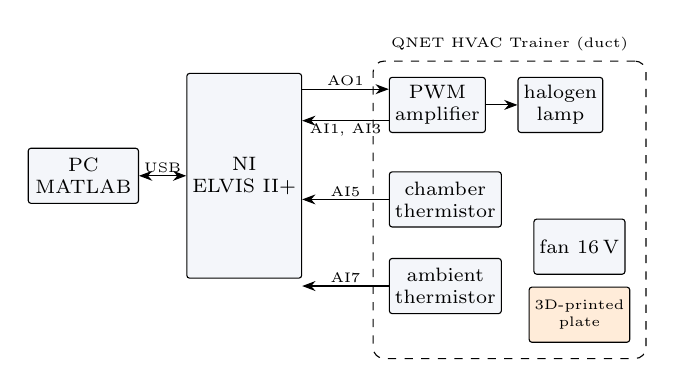
\begin{tikzpicture}[font=\scriptsize, >=Stealth]
\node[box, minimum width=14mm] (pc) {PC\\MATLAB};
\node[box, right=6mm of pc, minimum width=14mm, minimum height=26mm] (elvis) {NI\\ELVIS II+};
\node[box, right=11mm of elvis, yshift=9mm] (amp) {PWM\\amplifier};
\node[box, right=4mm of amp] (lamp) {halogen\\lamp};
\node[box, right=11mm of elvis, yshift=-3mm] (tc) {chamber\\thermistor};
\node[box, right=11mm of elvis, yshift=-14mm] (ta) {ambient\\thermistor};
\node[box, right=4mm of ta, yshift=5mm] (fan) {fan \SI{16}{V}};
\node[box, below=1.5mm of fan, font=\tiny, fill=orange!15] (plate) {3D-printed\\plate};
\draw[<->] (pc) -- node[above, lab]{USB} (elvis);
\draw[->] ([yshift=2mm]elvis.east |- amp) -- node[above, lab]{AO1} ([yshift=2mm]amp.west);
\draw[<-] ([yshift=-2mm]elvis.east |- amp) -- node[below, lab]{AI1, AI3} ([yshift=-2mm]amp.west);
\draw[->] (amp) -- (lamp);
\draw[->] (tc) -- node[above, lab]{AI5} (elvis.east |- tc);
\draw[->] (ta) -- node[above, lab]{AI7} (elvis.east |- ta);
\node[draw, dashed, rounded corners, fit=(amp)(lamp)(tc)(ta)(fan)(plate), inner sep=2mm,
      label={[font=\tiny]above:QNET HVAC Trainer (duct)}] {};
\end{tikzpicture}
\column{0.43\textwidth}
\small
\begin{itemize}
\item Duct with lamp heater, fixed-speed fan, chamber and ambient thermistors
\item MATLAB \(\leftrightarrow\) NI-DAQmx, \SI{2}{Hz} loop
\item Heater \SIrange{0}{5}{V}; current and voltage sensed
\item Safety: heater off above \SI{45}{\celsius} or ambient \(+\SI{20}{\celsius}\), on error, on exit
\end{itemize}
\end{columns}
\end{frame}

% ---------------------------------------------------------------
\begin{frame}{Fabricated parts: 3D-printed airflow plates}
\begin{columns}[c]
\column{0.5\textwidth}
\begin{itemize}
\item Fan speed is fixed \(\Rightarrow\) airflow changed with slip-on caps
\item Parametric OpenSCAD design: sleeve over the fan housing, face plate with a hole of a chosen open fraction \(f\), \(d=d_\mathrm{fan}\sqrt{f}\)
\item Three prints:
  \begin{itemize}
  \item \(f=1\): fit check
  \item \(f=0.5\): disturbance, restricted airflow
  \item \(f=0\): fan-failure emulation
  \end{itemize}
\item PETG/PLA, fan end only, \(\ge\)\SI{5}{cm} from the lamp
\end{itemize}
\column{0.46\textwidth}
\centering
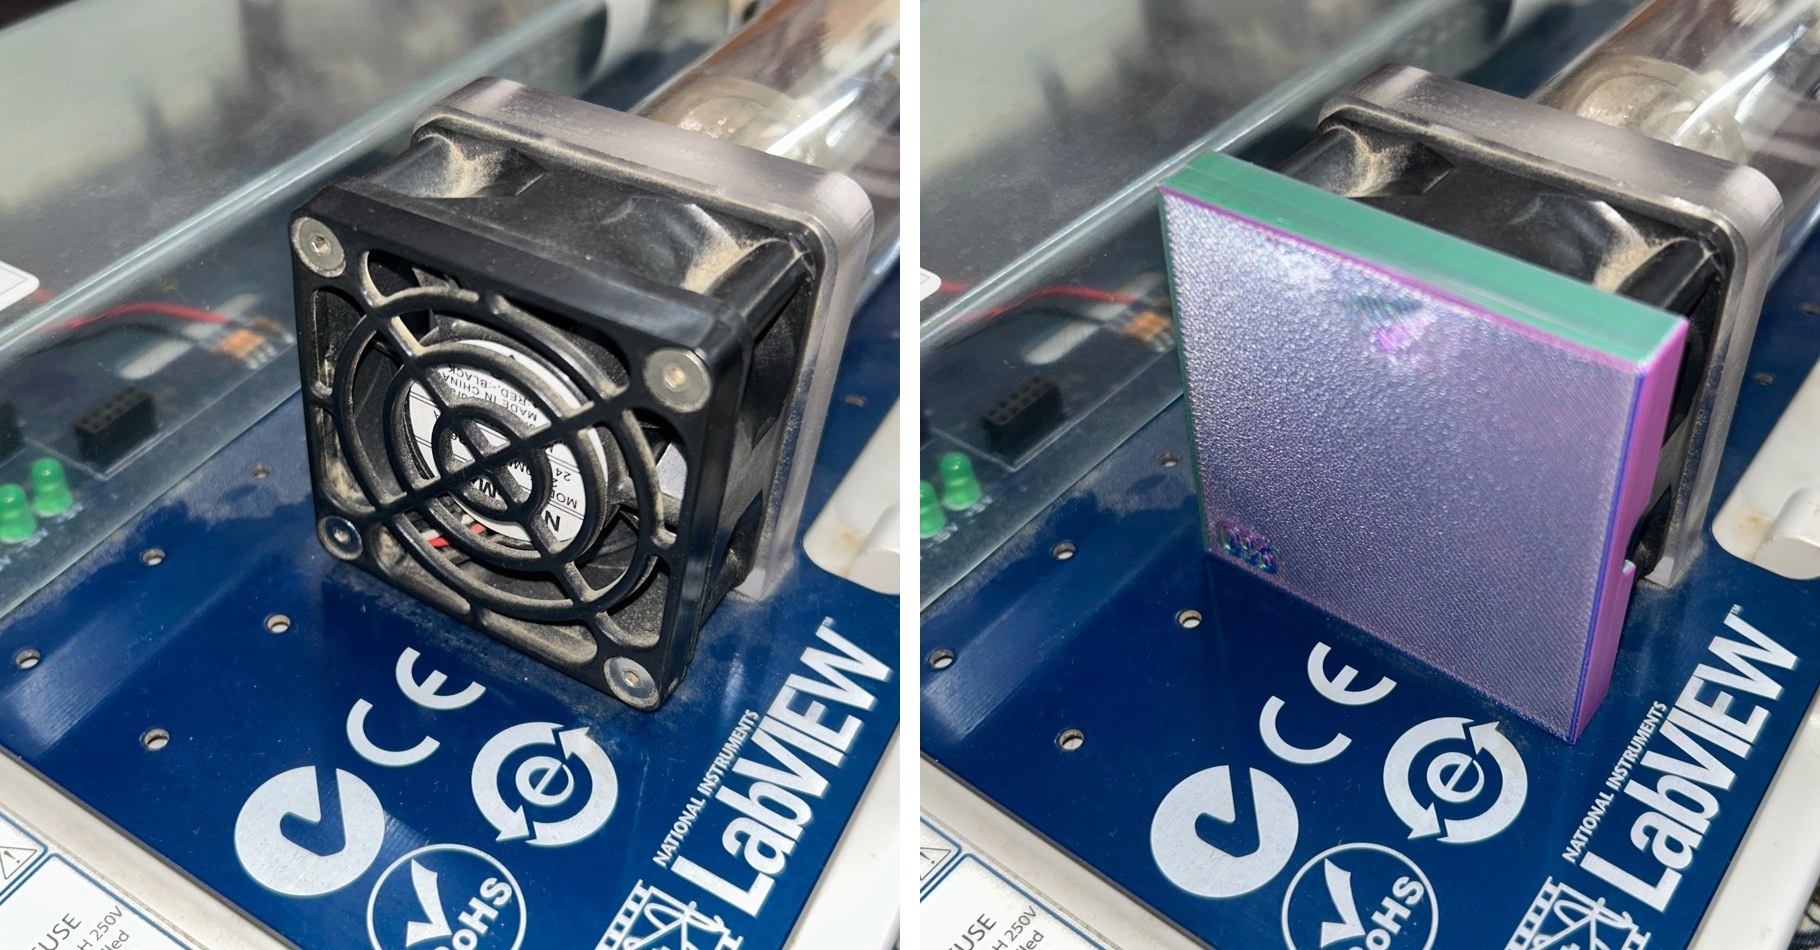
\includegraphics[width=\linewidth]{fan_plate_photos}\\[1mm]
\scriptsize fan without a plate (left) and with the closed 0\,\% plate fitted (right)
\end{columns}
\end{frame}

% ---------------------------------------------------------------
\begin{frame}{Thermal model and identification}
\begin{columns}[c]
\column{0.45\textwidth}
\[
\tau\,\dot T = K\,u(t-L) - a(t)\,(T-T_a)
\]
\small
heat in from the lamp \(-\) heat carried away by the airflow
\begin{itemize}
\item \(a=1\) normal airflow, \(a<1\) restricted
\item \SI{3}{V} open-loop step, output-error fit:\\
\(K=\SI{1.71}{\celsius\per\volt}\), \(\tau=\SI{33.7}{s}\), \(L\approx\SI{0.5}{s}\), fit 89\,\%
\item Refit on closed-loop data (detector model):\\ \(K=1.41\), \(\tau=\SI{19.6}{s}\)
\end{itemize}
\column{0.53\textwidth}
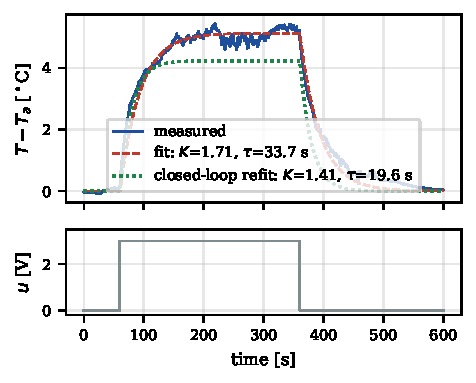
\includegraphics[width=\linewidth]{identification}
\end{columns}
\end{frame}

% ---------------------------------------------------------------
\begin{frame}{Simulink model}
\centering
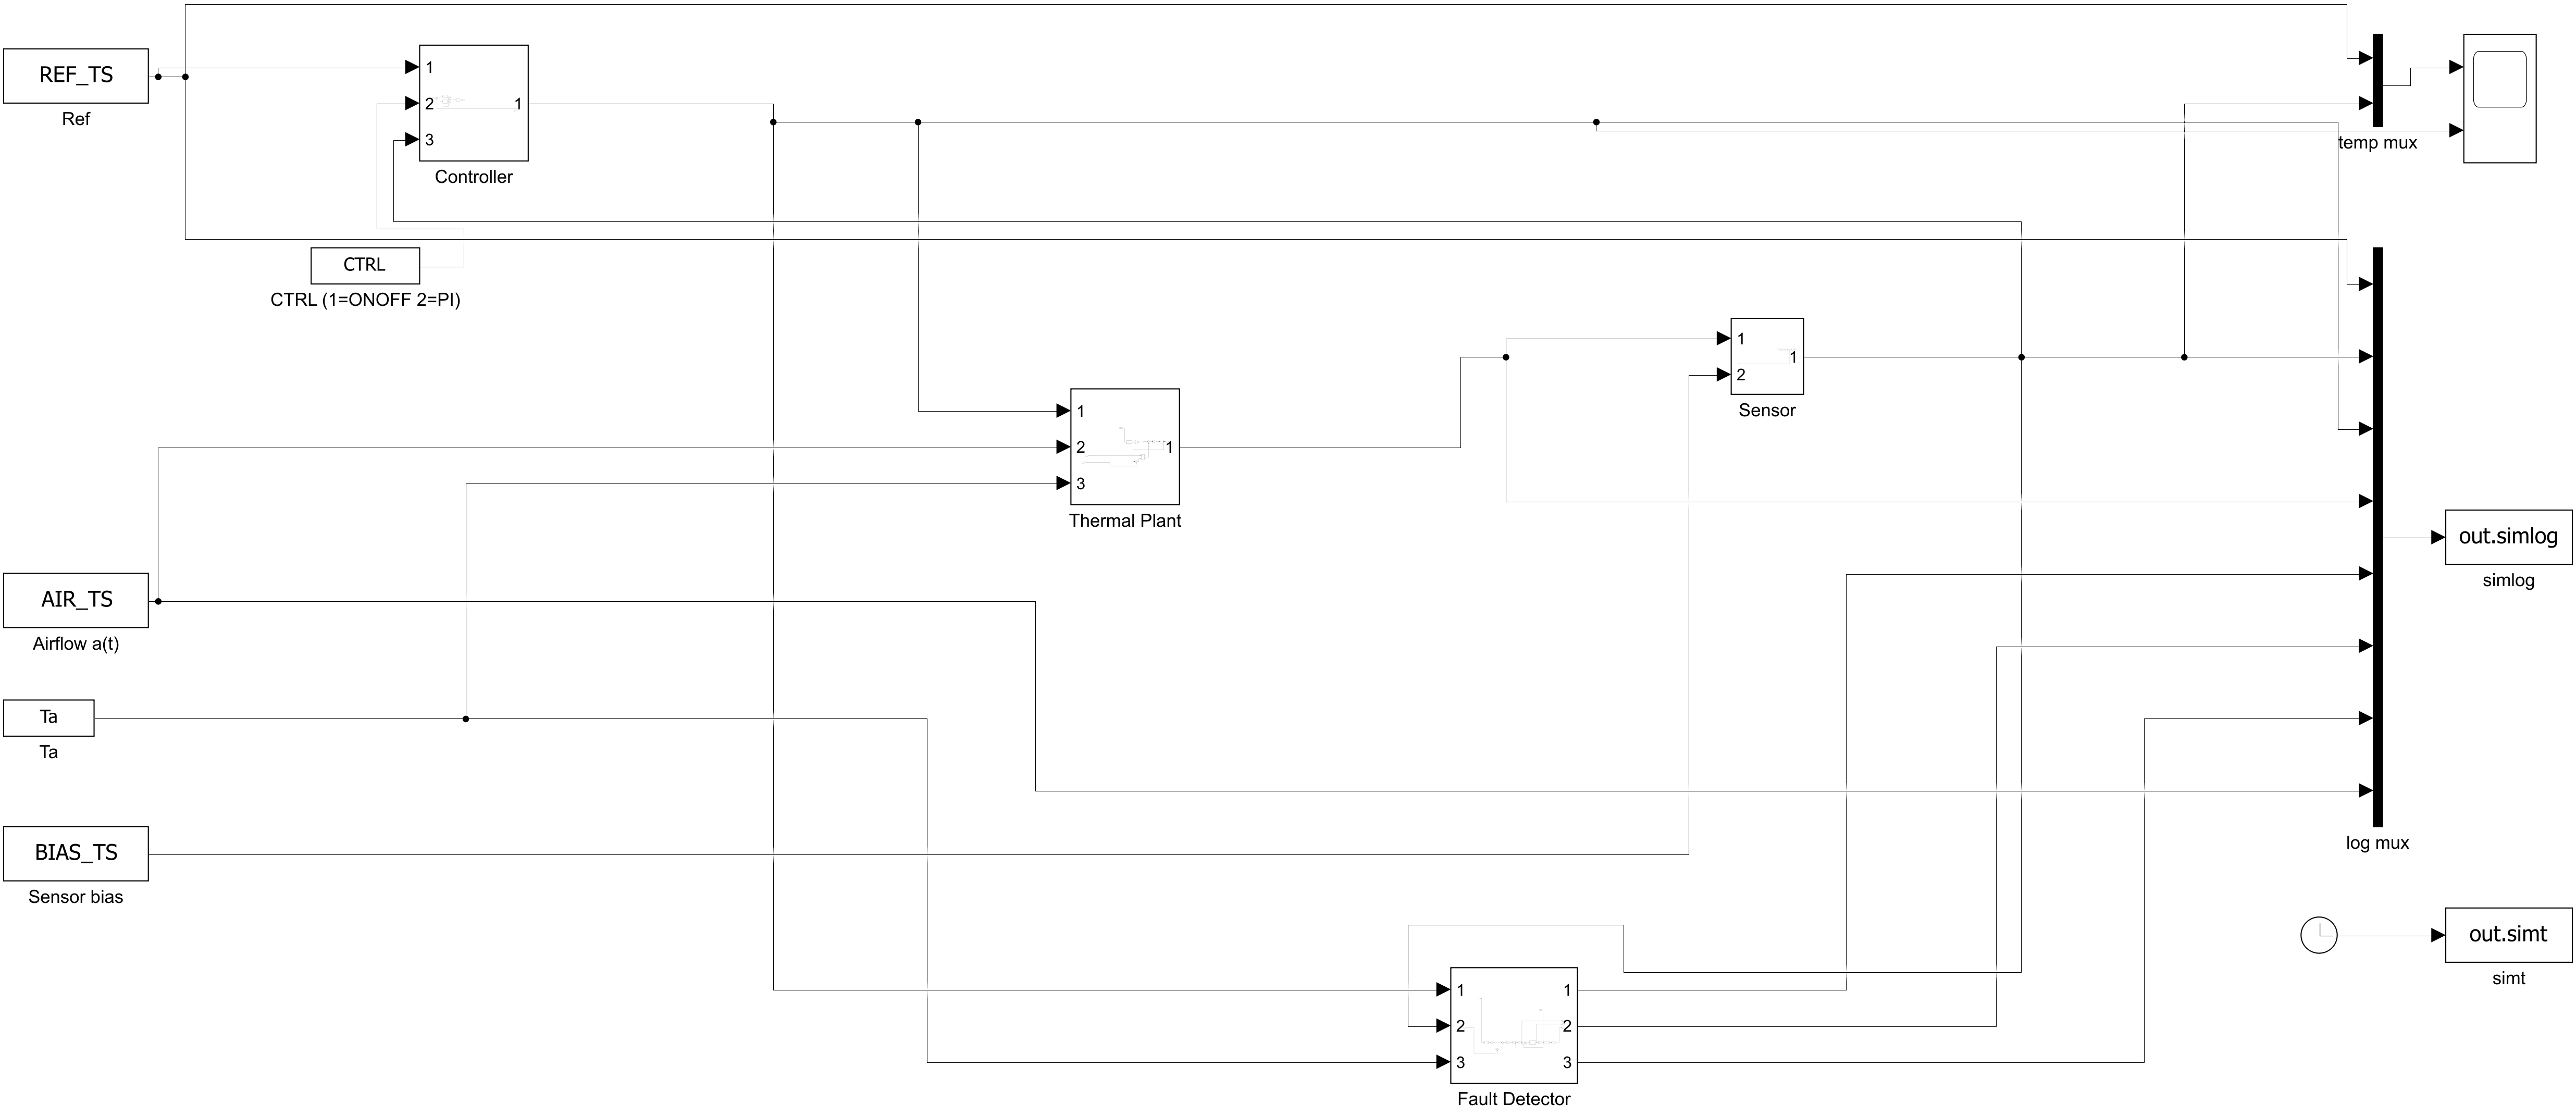
\includegraphics[width=\linewidth,height=0.74\textheight,keepaspectratio]{simulink}\\[1mm]
\small Controller \(\cdot\) thermal plant with airflow factor \(a(t)\) \(\cdot\) sensor lag and bias \(\cdot\) fault detector.
Every hardware run is replayed here with the logged inputs.
\end{frame}

\begin{frame}{Simulink model: thermal plant subsystem}
\centering
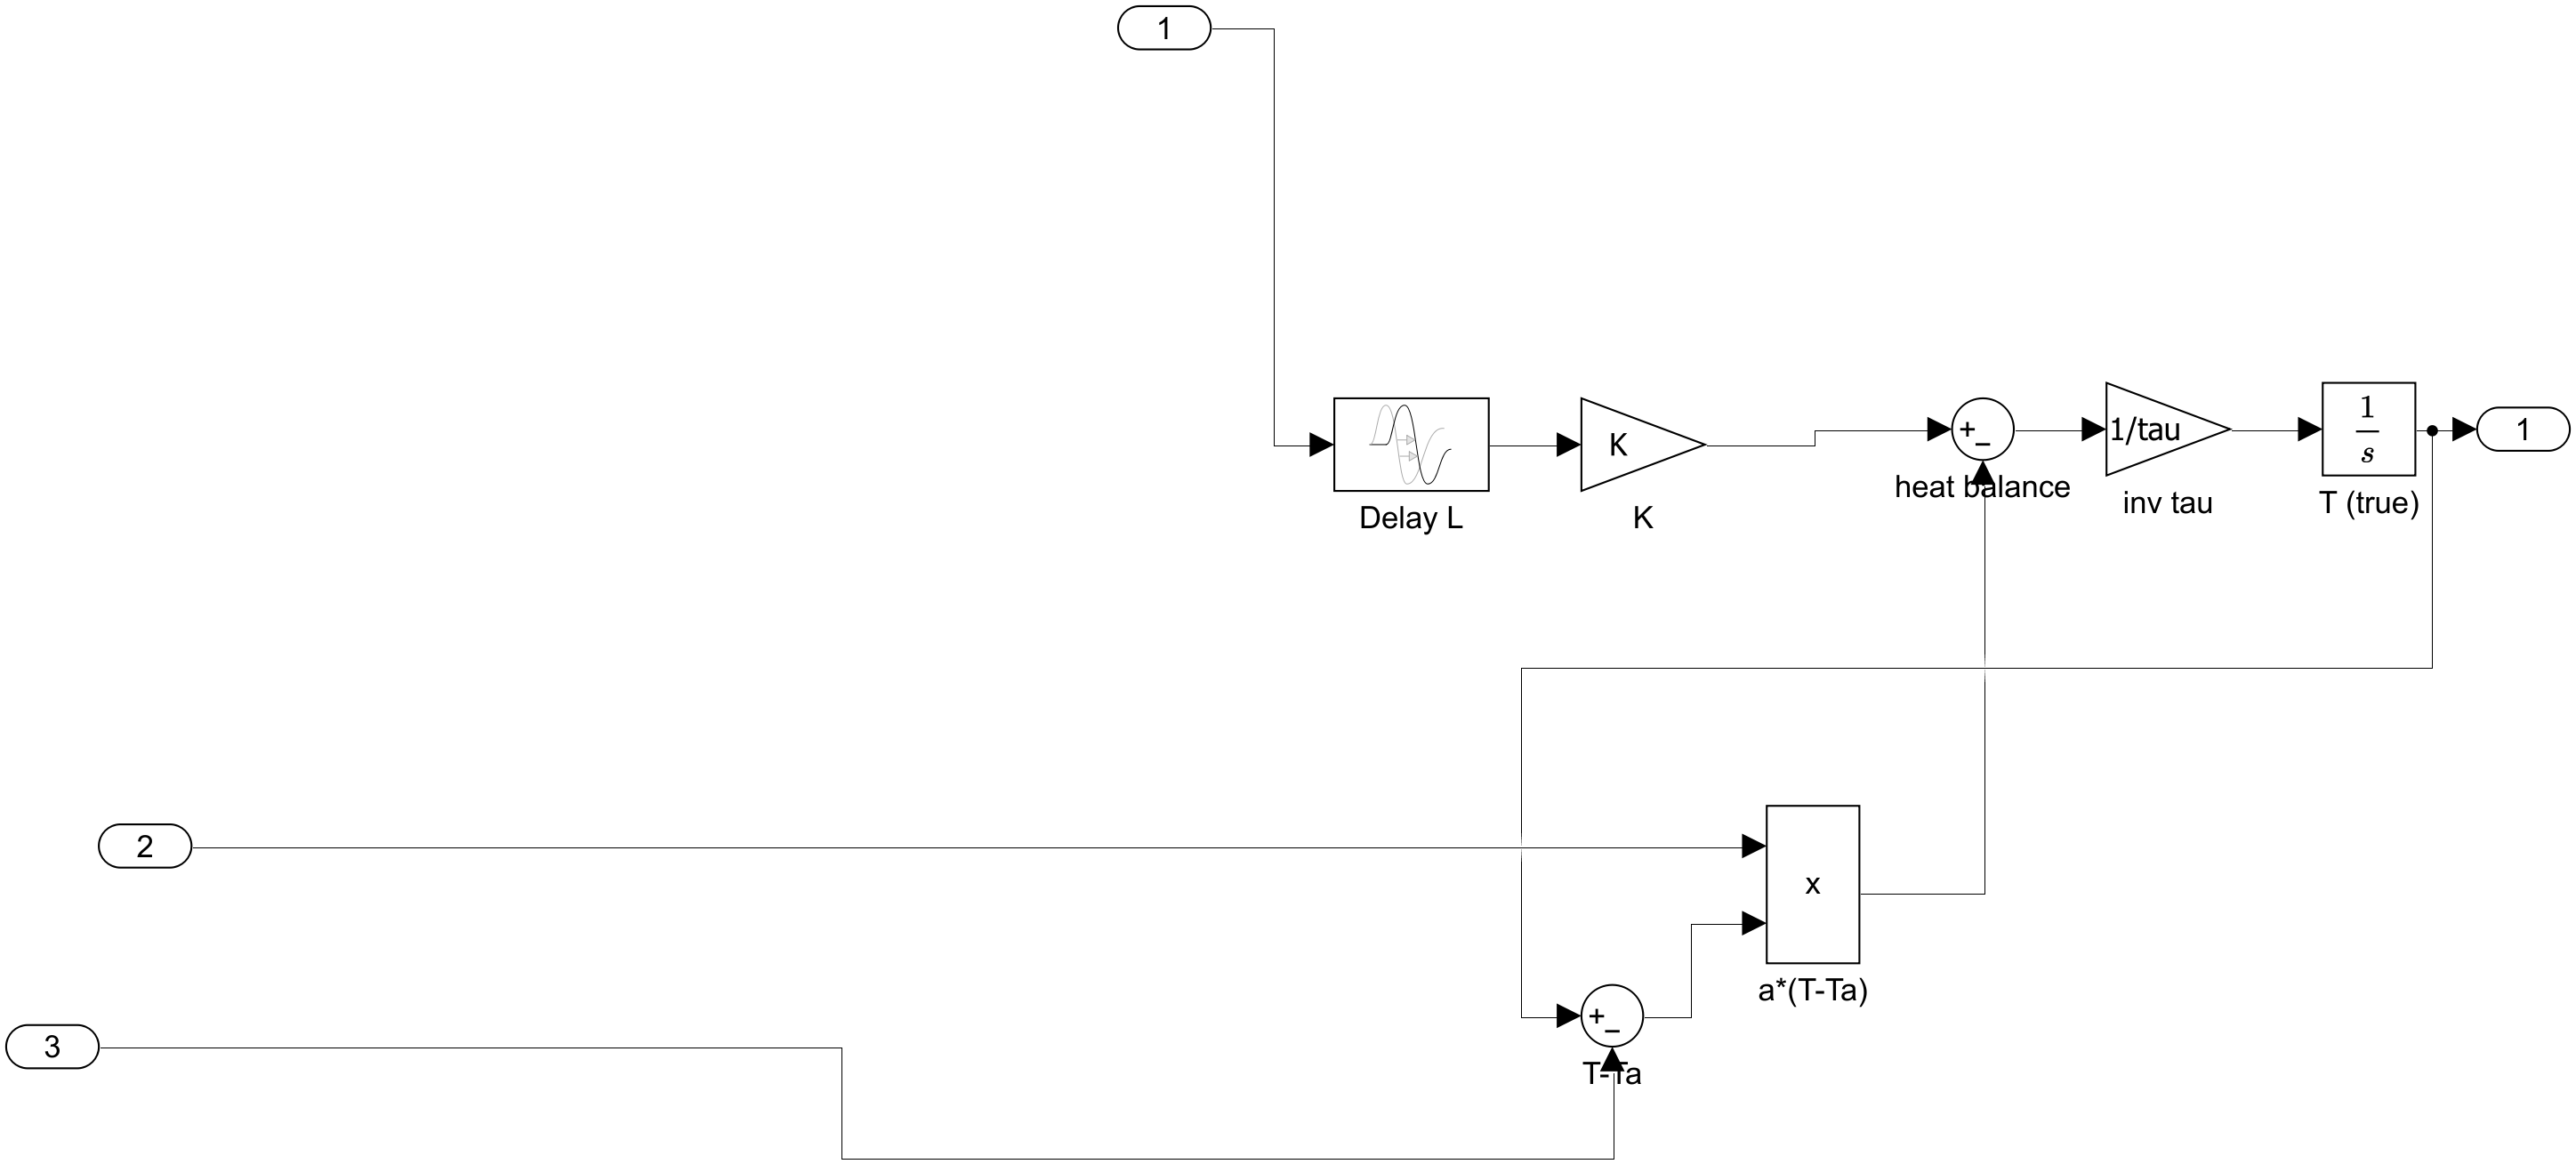
\includegraphics[width=0.9\linewidth,height=0.70\textheight,keepaspectratio]{simulink_plant}\\[1mm]
\small \(\tau\,\dot T = K\,u(t-L) - a(t)\,(T-T_a)\): delay \(L\), gain \(K\), heat balance, \(1/\tau\), integrator
\end{frame}

% ---------------------------------------------------------------
\begin{frame}{Controllers}
\begin{columns}[T]
\column{0.46\textwidth}
\textbf{ON-OFF with hysteresis}
\begin{itemize}
\item \SI{5}{V} when \(e>H/2\), \SI{0}{V} when \(e<-H/2\)
\item \(H=\SI{0.6}{\celsius}\)
\item Simple and fast, but a permanent limit cycle
\end{itemize}
\column{0.50\textwidth}
\textbf{PI, SIMC tuning}
\[
K_p=\frac{\tau}{K(\tau_c+L)},\quad T_i=\min\bigl(\tau,4(\tau_c+L)\bigr)
\]
\begin{itemize}
\item \(\tau_c=\tau/4\) \(\Rightarrow\) \(K_p=2.21\), \(T_i=\SI{33.7}{s}\)
\item Output limited to \SIrange{0}{5}{V}, clamping anti-windup
\end{itemize}
\end{columns}
\end{frame}

% ---------------------------------------------------------------
\begin{frame}{Fault detector}
\begin{columns}[c]
\column{0.52\textwidth}
\centering
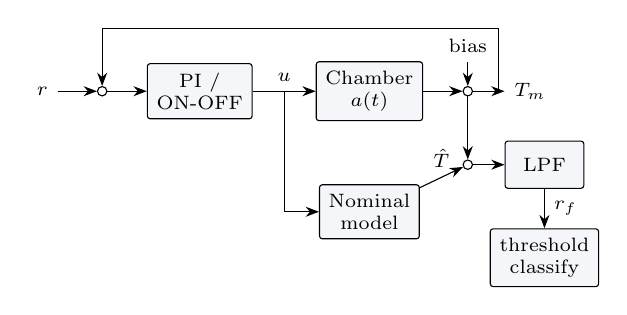
\begin{tikzpicture}[font=\scriptsize, >=Stealth, node distance=4mm and 5mm]
\node (ref) {$r$};
\node[sum, right=of ref] (s1) {};
\node[blk, right=of s1] (ctl) {PI /\\ON-OFF};
\node[blk, right=8mm of ctl] (plant) {Chamber\\$a(t)$};
\node[sum, right=of plant] (s2) {};
\node[right=4mm of s2] (y) {$T_m$};
\node[blk, below=8mm of plant] (mdl) {Nominal\\model};
\node[sum, below=8mm of s2] (s3) {};
\node[blk, right=4mm of s3] (lpf) {LPF};
\node[blk, below=5mm of lpf] (dec) {threshold\\classify};
\node[above=3mm of s2] (bias) {bias};
\draw[->] (ref) -- (s1); \draw[->] (s1) -- (ctl);
\draw[->] (ctl) -- node[above]{$u$} (plant); \draw[->] (plant) -- (s2);
\draw[->] (bias) -- (s2); \draw[->] (s2) -- (y);
\draw[->] ($(s2)!0.5!(y)$) |- ++(0,8mm) -| (s1);
\draw[->] ($(ctl)!0.5!(plant)$) |- (mdl);
\draw[->] (mdl) -- node[above]{$\hat T$} (s3);
\draw[->] (s2) -- (s3); \draw[->] (s3) -- (lpf); \draw[->] (lpf) -- node[right]{$r_f$} (dec);
\end{tikzpicture}
\column{0.46\textwidth}
\small
\begin{itemize}
\item Residual \(r=T_m-\hat T\), low-pass \(T_f=\SI{20}{s}\)
\item Alarm: \(|r_f|>\SI{1.3}{\celsius}\) for \SI{15}{s}
\item Classification
  \begin{itemize}
  \item jump \(>\SI{1}{\celsius}\)/sample \(\to\) \textbf{sensor bias}
  \item \(r_f>0\) \(\to\) \textbf{low airflow}
  \item \(r_f<0\) \(\to\) \textbf{excess cooling}
  \item no current with \(u>0.5\)\,V \(\to\) \textbf{heater fault}
  \end{itemize}
\item Same code in Simulink and on hardware
\end{itemize}
\end{columns}
\end{frame}

% ---------------------------------------------------------------
\begin{frame}{Setpoint tracking: hardware vs.\ simulation}
\centering
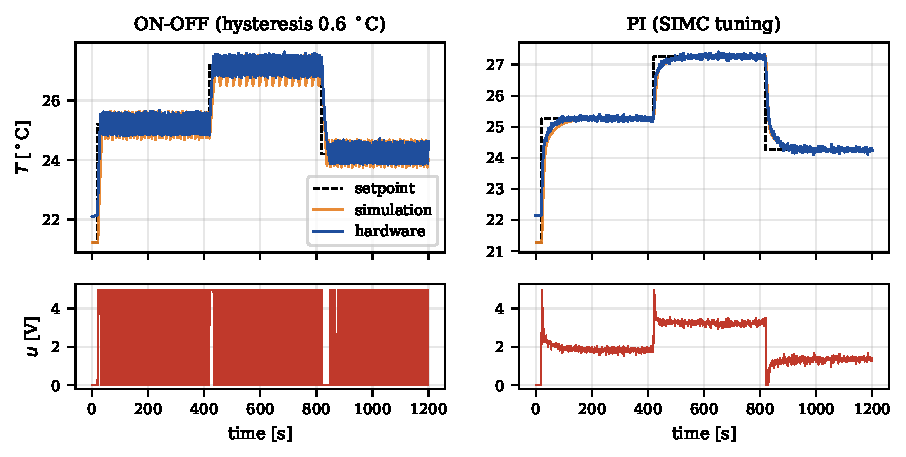
\includegraphics[width=0.92\linewidth]{tracking}\\[1mm]
\small ON-OFF: fastest rise, \(\approx\SI{0.8}{\celsius}\) limit cycle.\quad
PI: no limit cycle, negligible steady-state error.
\end{frame}

% ---------------------------------------------------------------
\begin{frame}{Tracking metrics}
\centering
{\small\begin{tabular}{@{}llccccc@{}}
\toprule
 & Step [$^\circ$C] & Rise [s] & Settle [s] & OS [\%] & $e_{ss}$ [$^\circ$C] & Ripple [$^\circ$C] \\
\midrule
ON-OFF & 0.0$\to$4.0 & 8.0 (13.0) & 7.5 (362.5) & 12.2 (11.4) & 0.00 (0.04) & 0.80 (0.97) \\
 & 4.0$\to$6.0 & 9.0 (16.0) & 7.5 (393.0) & 22.5 (16.3) & 0.00 (0.17) & 0.82 (1.01) \\
 & 6.0$\to$3.0 & 18.0 (10.5) & 207.0 (12.5) & 11.7 (15.0) & 0.01 (-0.02) & 0.78 (0.93) \\
\midrule
PI & 0.0$\to$4.0 & 24.0 (40.5) & 22.5 (34.5) & 3.3 (0.0) & 0.00 (0.00) & 0.22 (0.00) \\
 & 4.0$\to$6.0 & 27.0 (42.5) & 13.5 (16.5) & 7.7 (0.0) & 0.01 (0.00) & 0.23 (0.00) \\
 & 6.0$\to$3.0 & 36.5 (36.5) & 29.0 (20.5) & 5.7 (0.0) & 0.00 (0.00) & 0.27 (0.00) \\
\bottomrule
\end{tabular}
}
\vspace{3mm}

\small Hardware values, simulation in brackets; settling band \SI{\pm0.5}{\celsius}.\\[2mm]
Same mean command (\SI{2.23}{V} vs.\ \SI{2.25}{V}), but ON-OFF used \SI{1760}{J} vs.\ \SI{861}{J} for PI:
lamp power \(\propto V^2\), so full-voltage switching costs more energy.
\end{frame}

% ---------------------------------------------------------------
\begin{frame}{Disturbance: 50\,\% airflow plate at 400--800\,s}
\centering
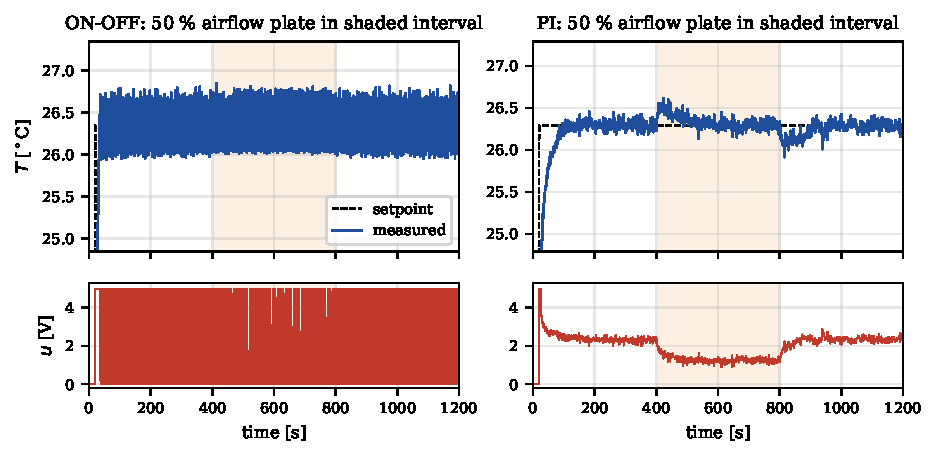
\includegraphics[width=0.92\linewidth]{disturbance}\\[1mm]
\small PI: peak \SI{0.32}{\celsius}, command \SI{2.4}{V}\(\to\)\SI{1.3}{V}.\quad
ON-OFF: peak \SI{0.50}{\celsius}, duty 47\,\%\(\to\)23\,\%.\quad
Both flagged \emph{low airflow} after \SIrange{30}{32}{s}.
\end{frame}

% ---------------------------------------------------------------
\begin{frame}{Fault detection under PI control}
\centering
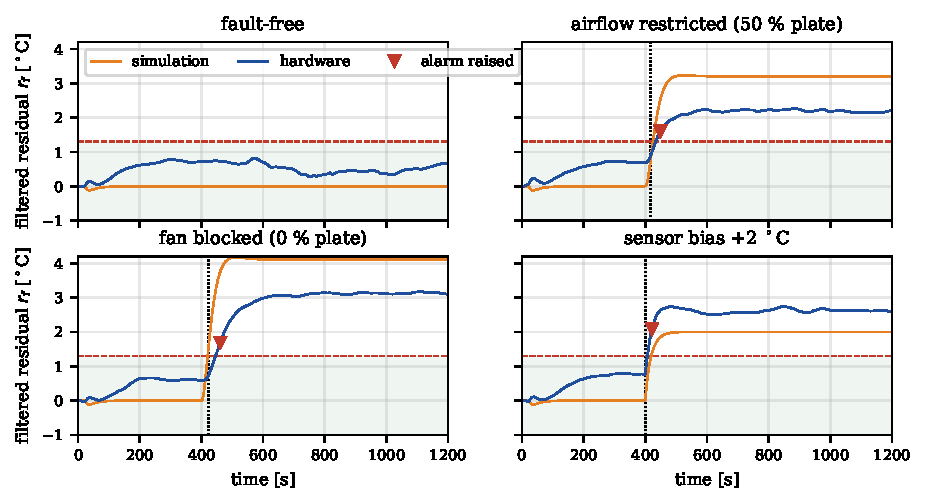
\includegraphics[width=0.85\linewidth]{faults}
\end{frame}

% ---------------------------------------------------------------
\begin{frame}{Fault detection: summary}
\centering
\begin{tabular}{@{}lccl@{}}
\toprule
Run & Fault at & Delay (sim) & Classified as \\
\midrule
Fault-free, PI          & --            & no alarm         & -- \\
Restricted 50\,\%, PI   & \SI{416.5}{s} & \SI{32.0}{s} (39.5) & low airflow \\
Blocked fan, PI         & \SI{422.5}{s} & \SI{38.5}{s} (35.0) & low airflow \\
Sensor bias, PI         & \SI{400.0}{s} & \SI{21.5}{s} (34.0) & sensor bias \\
Disturbance, ON-OFF     & \SI{404.5}{s} & \SI{32.0}{s}        & low airflow \\
Disturbance, PI         & \SI{406.5}{s} & \SI{30.0}{s}        & low airflow \\
\bottomrule
\end{tabular}

\vspace{4mm}
\small
\begin{itemize}
\item Fault-free residual peak \SI{0.82}{\celsius}: \SI{0.5}{\celsius} margin to the threshold
\item Airflow factor estimated from data: \(a\approx0.36\) (50\,\% plate), \(a\approx0.18\) (closed); used in the simulation
\end{itemize}
\end{frame}

% ---------------------------------------------------------------
\begin{frame}{Normal vs.\ faulted operation}
\centering
\small
\begin{tabular}{@{}lcccc@{}}
\toprule
PI run & $\bar u$ [V] & Duty [\%] & $|e|$ meas./true [$^\circ$C] & $E^\dagger$ [J] \\
\midrule
fault-free & 2.53 & 51 & 0.04 / 0.04 & 1059 \\
restricted 50\,\% & 1.29 & 26 & 0.04 / 0.04 & 473 \\
fan blocked & 0.68 & 14 & 0.07 / 0.07 & 398 \\
sensor bias & 1.19 & 24 & 0.03 / 2.00 & 492 \\
\bottomrule
\multicolumn{5}{@{}l}{\footnotesize $^\dagger$whole run; provisional current/voltage scaling}
\end{tabular}

\vspace{3mm}
\begin{itemize}
\item Airflow faults: heater effort drops to \(\sim\tfrac12\) and \(\sim\tfrac14\) at the same temperature
\item Sensor bias: the reading looks perfect, but the true chamber temperature is \SI{2}{\celsius} \emph{below} the setpoint
\item Neither shows up in the tracking error \(\to\) the residual is what reveals them
\end{itemize}
\end{frame}

% ---------------------------------------------------------------
\begin{frame}{Making the detector work on hardware}
\begin{columns}[c]
\column{0.5\textwidth}
\small
\textbf{1. Model gain.} The step-test model over-predicted closed-loop heating
(\(\sim\)\SI{1.3}{\celsius\per\volt} vs.\ 1.71) \(\to\) residual drifted to
\SI{-2.4}{\celsius}, false \emph{excess cooling}.\\
Fix: refit \(K,\tau\) on closed-loop data.\\[3mm]
\textbf{2. Resting reference.} The heater-off chamber reading sat
\SIrange{-0.2}{+1.0}{\celsius} from the ambient sensor, varying by session
\(\to\) false \emph{low airflow}.\\
Fix: the model relaxes to the chamber's own starting value; runs start from a cooled chamber.
\column{0.48\textwidth}
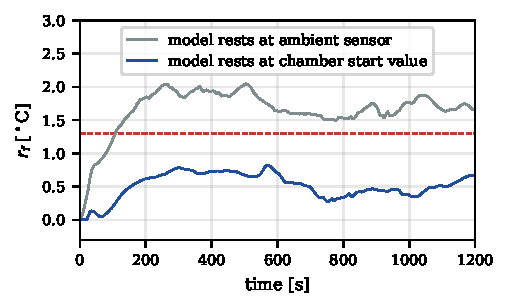
\includegraphics[width=\linewidth]{rest_fix}\\
\centering\scriptsize fault-free run: peak residual \SI{2.05}{\celsius}\(\to\)\SI{0.82}{\celsius}
\end{columns}
\end{frame}

% ---------------------------------------------------------------
\begin{frame}{Limitations}
\begin{itemize}
\item Single-node model of a distributed duct; lamp power is not linear in the command
\item Fixed-speed fan: airflow changes only in discrete plate steps
\item Sensor bias injected in software
\item Ambient drift and a session-dependent resting offset; runs must start from a cooled chamber
\item Heater current/voltage scalings provisional \(\to\) joule values approximate
\item Sensor-fault label reverts to the sign test after \SI{90}{s}; heater fault not staged
\end{itemize}
\end{frame}

% ---------------------------------------------------------------
\begin{frame}{Conclusions}
\begin{itemize}
\item PI (SIMC from one step test) tracks smoothly, settles in \SIrange{13.5}{29}{s}, holds the chamber
within \SI{0.35}{\celsius} through airflow faults and uses about half the energy; ON-OFF keeps a
\(\sim\)\SI{0.8}{\celsius} limit cycle
\item The residual detector catches and classifies all three faults in \SIrange{21.5}{38.5}{s},
with no false alarm in the fault-free run
\item Hardware and simulation agree once the airflow factors are estimated from data
\item Next: adaptive or observer-based residual, latched fault labels, online airflow estimate
\end{itemize}
\vspace{5mm}
\centering
\textbf{Live demo:} PI disturbance run \(\to\) insert the plate \(\to\) recovery and \emph{low airflow} alarm
\(\to\) press \texttt{b} \(\to\) \emph{sensor bias} alarm
\end{frame}

\end{document}
